\mfpicnumber{1}

\opengraphsfile{ExpEquations}

\setcounter{footnote}{0}

\label{ExpEquations}

In this section we will develop techniques for solving equations involving exponential functions.  Suppose, for instance,  we wanted to solve the equation $2^{x} = 128$.  After a moment's calculation, we find $128 = 2^{7}$, so we have $2^{x} = 2^{7}$.  The one-to-one property of exponential functions, detailed in Theorem \ref{explogsonetoone}, tells us that $2^{x} = 2^{7}$ if and only if $x=7$.  This means that not only is $x=7$ a solution to $2^{x} = 2^{7}$, it is the \textit{only} solution.  Now suppose we change the problem ever so slightly to $2^{x} = 129$.  We could use one of the inverse properties of exponentials and logarithms listed in Theorem \ref{invpropslogs} to write $129 = 2^{\log_{2}(129)}$.  We'd then have $2^{x} = 2^{\log_{2}(129)}$, which means our solution is $x = \log_{2}(129)$. This makes sense because, after all, the definition of $\log_{2}(129)$ is `the exponent we put on $2$ to get $129$.' Indeed we could have obtained this solution directly by rewriting the equation $2^{x} = 129$ in its logarithmic form $\log_{2}(129) = x$.  Either way, in order to get a reasonable decimal approximation to this number, we'd use the change of base formula, Theorem \ref{changeofbase}, to give us something more calculator friendly,\footnote{You can use natural logs or common logs.  We choose natural logs.  (In Calculus, you'll learn these are the most `mathy' of the logarithms.)} say $\log_{2}(129) = \frac{\ln(129)}{\ln(2)}$.  Another way to arrive at this answer is as follows


\[ \begin{array}{rclr}
2^{x} & = & 129 & \\
\ln\left(2^{x}\right) & = & \ln(129) & \mbox{Take the natural log of both sides.} \\
x \ln(2) & = & \ln(129) & \mbox{Power Rule} \\ [4pt]
x & = &\dfrac{\ln(129)}{\ln(2)} & \\
\end{array}\]

`Taking the natural log' of both sides is akin to squaring both sides: since $f(x) = \ln(x)$ is a \textit{function}, as long as two quantities are equal, their natural logs are equal.\footnote{This is also the `if' part of the statement $\log_{b}(u) = \log_{b}(w)$ if and only if $u=w$ in Theorem \ref{explogsonetoone}.} Also note that we treat $\ln(2)$ as any other non-zero real number and divide it through\footnote{Please resist the temptation to divide both sides by `$\ln$' instead of $\ln(2)$.   Just like it wouldn't make sense to divide both sides by the square root symbol `$\sqrt{\vphantom{2} \,}$' when solving $x \sqrt{2} = 5$, it makes no sense to divide by `$\ln$'.}  to isolate the variable $x$.  We summarize below the two common ways to solve exponential equations, motivated by our examples.

\smallskip

\colorbox{ResultColor}{\bbm

\centerline{\textbf{Steps for Solving an Equation involving Exponential Functions}} \index{exponential function ! solving equations with}

\begin{enumerate}

\item  Isolate the exponential function.

\item  

\begin{enumerate}

\item  If convenient, express both sides with a common base and equate the exponents.

\item  Otherwise, take the natural log of both sides of the equation and use the Power Rule.


\end{enumerate}


\end{enumerate}

\ebm}

\smallskip


\begin{ex}  \label{expeqnsex1} Solve the following equations.  Check your answer graphically using a calculator.

\begin{multicols}{3}
\begin{enumerate}

\item  $2^{3x} = 16^{1-x}$

\item  $2000 = 1000 \cdot 3^{-0.1 t}$ 

\item  $9 \cdot 3^{x} = 7^{2x}$

\setcounter{HW}{\value{enumi}}
\end{enumerate}
\end{multicols}

\begin{multicols}{3}
\begin{enumerate}
\setcounter{enumi}{\value{HW}}

\item  $75 = \frac{100}{1 + 3e^{-2t}}$

\item  $25^{x} = 5^{x} + 6$

\item  $\frac{e^{x} - e^{-x}}{2} = 5$

\end{enumerate}
\end{multicols}

{\bf Solution.}

\begin{enumerate}

\item  Since $16$ is a power of $2$, we can rewrite  $2^{3x} =  16^{1-x}$ as $2^{3x} = \left(2^4\right)^{1-x}$.  Using properties of exponents, we get $2^{3x} = 2^{4(1-x)}$.  Using the one-to-one property of exponential functions, we get $3x = 4(1-x)$ which gives $x=\frac{4}{7}$. To check graphically, we set $f(x) = 2^{3x}$ and $g(x) = 16^{1-x}$ and see that they intersect at $x=\frac{4}{7} \approx 0.5714$.

\item  We begin solving $2000 = 1000 \cdot 3^{-0.1 t}$  by dividing both sides by $1000$ to isolate the exponential which yields $3^{-0.1t} = 2$.  Since it is inconvenient to write $2$ as a power of $3$, we use the natural log to get $\ln\left(3^{-0.1t}\right) = \ln(2)$.  Using the Power Rule, we get $-0.1 t \ln(3) = \ln(2)$, so we divide both sides by $-0.1 \ln(3)$ to get $t = -\frac{\ln(2)}{0.1 \ln(3)} = -\frac{10\ln(2)}{\ln(3)}$.  On the calculator, we graph $f(x) = 2000$ and $g(x) =  1000 \cdot 3^{-0.1 x}$ and find that they intersect at $x = -\frac{10\ln(2)}{\ln(3)} \approx -6.3093$.

\begin{center}

\begin{tabular}{cc}

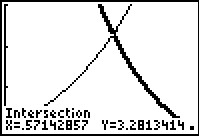
\includegraphics[width=2in]{./ExpLogsGraphics/ExpEqns01.jpg} &

\hspace{0.75in} 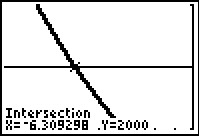
\includegraphics[width=2in]{./ExpLogsGraphics/ExpEqns02.jpg} \\

$y = f(x) =2^{3x}$ and  & 

 \hspace{0.75in}  $y = f(x) = 2000$ and  \\
 
 \boldmath $y=g(x) =16^{1-x}$ & \hspace{0.75in} \boldmath $y=g(x) = 1000 \cdot 3^{-0.1 x}$\\
 
\end{tabular}

\end{center}

\item  We first note that we can rewrite the equation $9 \cdot 3^{x} = 7^{2x}$ as $3^2 \cdot 3^x = 7^{2x}$ to obtain $3^{x+2} = 7^{2x}$.  Since it is not convenient to express both sides as a power of $3$ (or $7$ for that matter) we use the natural log:  $\ln\left(3^{x+2}\right) = \ln\left(7^{2x}\right)$.  The power rule gives $(x+2) \ln(3) = 2x \ln(7)$.  Even though this equation appears very complicated, keep in mind that $\ln(3)$ and $\ln(7)$ are just constants.  The equation $(x+2) \ln(3) = 2x \ln(7)$ is actually a linear equation and as such we gather all of the terms with $x$ on one side, and the constants on the other.  We then divide both sides by the coefficient of $x$, which we obtain by factoring.

\[ \begin{array}{rclr}
(x+2) \ln(3) & = & 2x \ln(7) & \\

x \ln(3) + 2 \ln(3) & = & 2x \ln(7) & \\
2 \ln(3) & = & 2x \ln(7) - x \ln(3) & \\
2 \ln(3) & = & x (2 \ln(7) - \ln(3)) & \mbox{Factor.}\\
x & = & \frac{2 \ln(3)}{2\ln(7) - \ln(3)} & \\ [4pt]
\end{array}\]

Graphing $f(x) = 9 \cdot 3^{x}$ and $g(x) = 7^{2x}$ on the calculator, we see that these two graphs intersect at $x = \frac{2 \ln(3)}{2\ln(7) - \ln(3)}  \approx 0.7866$.

\item  Our objective in solving  $75 = \frac{100}{1 + 3e^{-2t}}$ is to first isolate the exponential.  To that end, we clear denominators and get $75\left(1 + 3e^{-2t}\right) = 100$. From this we get $75 + 225e^{-2t} =100$, which leads to  $225e^{-2t} = 25$, and finally, $e^{-2t} = \frac{1}{9}$.    Taking the natural log of both sides gives $\ln\left(e^{-2t}\right) = \ln\left( \frac{1}{9} \right)$.  Since natural log is log base $e$, $\ln\left(e^{-2t}\right) = -2t$.  We can also use the Power Rule to write $\ln\left( \frac{1}{9} \right) = -\ln(9)$.  Putting these two steps together, we simplify $\ln\left(e^{-2t}\right) = \ln\left( \frac{1}{9} \right)$ to   $-2t = -\ln(9)$.  We arrive at our solution, $t = \frac{\ln(9)}{2}$ which simplifies to $t = \ln(3)$. (Can you explain why?)  The calculator confirms the graphs of $f(x) = 75$ and $g(x) = \frac{100}{1 + 3e^{-2x}}$ intersect at $x = \ln(3) \approx 1.099$.

\begin{center}

\begin{tabular}{cc}

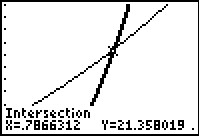
\includegraphics[width=2in]{./ExpLogsGraphics/ExpEqns03.jpg} &

\hspace{0.75in} 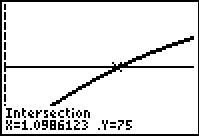
\includegraphics[width=2in]{./ExpLogsGraphics/ExpEqns04.jpg} \\

$y = f(x) = 9 \cdot 3^{x} $ and   & 

 \hspace{0.75in}  $y = f(x) = 75$ and \\
 
 \boldmath $y=g(x) = 7^{2x}$ & 
 \hspace{0.75in} \boldmath $y=g(x) = \frac{100}{1 + 3e^{-2x}}$  \\

\end{tabular}

\end{center}

\item  We start solving $25^{x} = 5^{x} + 6$ by rewriting $25 = 5^2$ so that we have $\left(5^2\right)^{x} = 5^{x} + 6$, or $5^{2x} = 5^{x} + 6$.  Even though we have a common base, having two terms on the right hand side of the equation foils our plan of equating exponents or taking logs.  If we stare at this long enough, we notice that we have three terms with the exponent on one term exactly twice that of another. To our surprise and delight, we have a  `quadratic in disguise'.  Letting $u = 5^{x}$,  we have $u^2 = \left(5^{x}\right)^2 = 5^{2x}$ so the equation $5^{2x} = 5^{x} + 6$ becomes $u^2 = u + 6$.  Solving this as $u^2 - u - 6=0$ gives $u = -2$ or $u = 3$.  Since $u = 5^{x}$, we have $5^{x} = -2$ or $5^{x} = 3$.  Since $5^{x} = -2$ has no real solution, (Why not?) we focus on $5^{x} = 3$.  Since it isn't convenient to express $3$ as a power of $5$, we take natural logs and get $\ln\left(5^{x}\right) = \ln(3)$ so that $x \ln(5) = \ln(3)$ or $x = \frac{\ln(3)}{\ln(5)}$.  On the calculator, we see the graphs of $f(x) = 25^{x}$ and $g(x) = 5^{x} + 6$ intersect at $x=\frac{\ln(3)}{\ln(5)} \approx 0.6826$.

\item  At first, it's unclear how to proceed with $\frac{e^{x} - e^{-x}}{2} = 5$, besides clearing the denominator to obtain $e^{x} - e^{-x} = 10$.  Of course, if we rewrite $e^{-x} = \frac{1}{e^{x}}$, we see we have another denominator lurking in the problem:  $e^{x} - \frac{1}{e^{x}} = 10$. Clearing this denominator gives us $e^{2x} - 1 = 10e^{x}$, and once again, we have an equation with three terms where the exponent on one term is exactly twice that of another - a `quadratic in disguise.'  If we let $u = e^{x}$, then $u^2 = e^{2x}$ so the equation $e^{2x} - 1 = 10e^{x}$ can be viewed as $u^2-1 = 10u$.  Solving $u^2 - 10u - 1 = 0$, we obtain by the quadratic formula $u = 5 \pm \sqrt{26}$.  From this, we have $e^{x} = 5 \pm \sqrt{26}$.  Since $5 - \sqrt{26} < 0$, we get no real solution to $e^{x} = 5 - \sqrt{26}$, but for $e^{x} = 5 + \sqrt{26}$, we take natural logs to obtain $x = \ln\left(5 + \sqrt{26}\right)$.  If we graph $f(x) = \frac{e^{x} - e^{-x}}{2}$ and $g(x) = 5$, we see that the graphs intersect at $x = \ln\left(5 + \sqrt{26}\right) \approx 2.312$

\begin{center}

\begin{tabular}{cc}

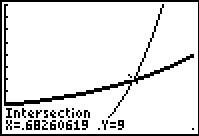
\includegraphics[width=2in]{./ExpLogsGraphics/ExpEqns05.jpg} &

\hspace{0.75in} 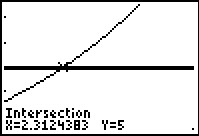
\includegraphics[width=2in]{./ExpLogsGraphics/ExpEqns06.jpg} \\

$y = f(x) = 25^{x}  $ and   & 

 \hspace{0.75in}  $y = f(x) = \frac{e^{x} - e^{-x}}{2}$ and \\
 
 \boldmath $y=g(x) = 5^{x} + 6$ & 
 \hspace{0.75in} \boldmath $y=g(x) = 5$  \\

\end{tabular}

\end{center}

\end{enumerate}

\qed

\end{ex}

The authors would be remiss not to mention that Example \ref{expeqnsex1} still holds great educational value.  Much can be learned about logarithms and exponentials by verifying the solutions obtained in Example \ref{expeqnsex1} analytically. For example, to verify our solution to  $2000 = 1000 \cdot 3^{-0.1 t}$, we substitute $t = -\frac{10\ln(2)}{\ln(3)}$ and obtain 
\[ \begin{array}{rclr}

2000 & \stackrel{?}{=} & 1000 \cdot 3^{-0.1 \left(-\frac{10\ln(2)}{\ln(3)}\right)} & \\
2000 & \stackrel{?}{=} & 1000 \cdot 3^{\frac{\ln(2)}{\ln(3)}} & \\
2000 & \stackrel{?}{=} & 1000 \cdot 3^{\log_{3}(2)} & \mbox{Change of Base}\\
2000 & \stackrel{?}{=} & 1000 \cdot 2 & \mbox{Inverse Property}\\
2000 & \stackrel{\checkmark}{=} & 2000 & \\

\end{array}\]

The other solutions can be verified by using a combination of log and inverse properties.  Some fall out quite quickly, while others are more involved.  We leave them to the reader.

\smallskip

Since exponential functions are continuous on their domains, the Intermediate Value Theorem \ref{IVT} applies.  As with the algebraic functions in Section \ref{AlgebraicFunctions}, this allows us to solve inequalities using sign diagrams as demonstrated below.

\begin{ex}  Solve the following inequalities.  Check your answer graphically using a calculator.
\label{expineq}

\begin{multicols}{3}

\begin{enumerate}

\item  $2^{x^2-3x} - 16 \geq 0$

\item  $\dfrac{e^{x}}{e^{x}-4} \leq 3$

\item  $x e^{2x} < 4x$

\end{enumerate}

\end{multicols}

{\bf Solution.}

\begin{enumerate}

\item  Since we already have $0$ on one side of the inequality, we set $r(x) = 2^{x^2-3x} - 16$.  The domain of $r$ is all real numbers, so in order to construct our sign diagram, we need to find the zeros of $r$.  Setting $r(x) = 0$ gives $2^{x^2-3x} - 16 = 0$ or $2^{x^2-3x} = 16$.  Since $16 = 2^{4}$ we have $2^{x^2-3x} = 2^{4}$, so by the one-to-one property of exponential functions, $x^2 -3x = 4$.  Solving $x^2 -3x - 4 = 0$ gives $x=4$ and $x=-1$.  From the sign diagram, we see $r(x) \geq 0$ on $(-\infty, -1] \cup [4, \infty)$, which corresponds to where the graph of  $y=r(x) = 2^{x^2-3x} - 16$, is on or above the $x$-axis.

\begin{center}

\begin{tabular}{m{2in}c}

\begin{mfpic}[10]{-5}{5}{-1}{2}
\arrow \reverse \arrow \polyline{(-5,0),(5,0)}
\xmarks{-2,2}
\tlabel[cc](-3.5,1){$(+)$}
\tlabel[cc](-2,-1){$-1$}
\tlabel[cc](-2,1){$0$}
\tlabel[cc](0,1){$(-)$}
\tlabel[cc](2,-1){$4$}
\tlabel[cc](2,1){$0$}
\tlabel[cc](3.5,1){$(+)$}
\end{mfpic}

& 

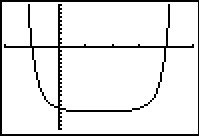
\includegraphics[width=2in]{./ExpLogsGraphics/ExpEqns07.jpg} \\

& $y=r(x) = 2^{x^2-3x} - 16$ \\

\end{tabular}

\end{center}

\item The first step we need to take to solve  $\frac{e^{x}}{e^{x}-4} \leq 3$ is to get $0$ on one side of the inequality. To that end, we subtract $3$ from both sides and get a common denominator


\setlength{\extrarowheight}{12pt}
\[ \begin{array}{rclr}

\dfrac{e^{x}}{e^{x}-4} & \leq & 3 & \\

\dfrac{e^{x}}{e^{x}-4} - 3 & \leq & 0 & \\

\dfrac{e^{x}}{e^{x}-4} - \dfrac{3 \left(e^{x}-4\right)}{e^{x}-4} & \leq & 0 & \mbox{Common denomintors.} \\

\dfrac{12 - 2e^{x}}{e^{x}-4} & \leq & 0 & \\

\end{array}\]
\setlength{\extrarowheight}{2pt}

We set $r(x) = \frac{12 - 2e^{x}}{e^{x}-4}$ and we note that $r$ is undefined when its denominator $e^{x}-4=0$, or when $e^{x} = 4$.  Solving this gives $x = \ln(4)$, so the domain of $r$ is $(-\infty, \ln(4)) \cup (\ln(4), \infty)$. To find the zeros of $r$, we solve $r(x) = 0$ and obtain $12 - 2e^{x} = 0$.  Solving for $e^{x}$, we find $e^{x} = 6$, or $x = \ln(6)$.  When we build our sign diagram, finding test values may be a little tricky since we need to check values around $\ln(4)$ and $\ln(6)$.  Recall that the function $\ln(x)$ is increasing\footnote{This is because the base of $\ln(x)$ is $e > 1$.  If the base $b$ were in the interval $0 < b < 1$, then $\log_{b}(x)$ would decreasing.} which means $\ln(3) < \ln(4) < \ln(5) < \ln(6) < \ln(7)$.  While the prospect of determining the sign of $r\left(\ln(3)\right)$ may be very unsettling, remember that $e^{\ln(3)} = 3$, so \[r\left(\ln(3)\right) = \frac{12 - 2e^{\ln(3)}}{e^{\ln(3)}-4} = \frac{12-2(3)}{3-4} = -6\]  We determine the signs of $r\left(\ln(5)\right)$ and $r\left(\ln(7)\right)$ similarly.\footnote{We could, of course, use the calculator, but what fun would that be?} From the sign diagram, we find our answer to be $(-\infty,\ln(4)) \cup [\ln(6), \infty)$.  Using the calculator, we see the graph of $f(x) = \frac{e^{x}}{e^{x}-4}$ is below the graph of $g(x) = 3$ on $(-\infty,\ln(4)) \cup (\ln(6), \infty)$, and they intersect at $x = \ln(6) \approx 1.792$.


\begin{center}

\begin{tabular}{m{2in}c}

\begin{mfpic}[10]{-5}{5}{-1}{2}
\arrow \reverse \arrow \polyline{(-5,0),(5,0)}
\xmarks{-2,2}
\tlabel[cc](-3.5,1){$(-)$}
\tlabel[cc](-2,-1){$\ln(4)$}
\tlabel[cc](-2,1){\textinterrobang}
\tlabel[cc](0,1){$(+)$}
\tlabel[cc](2,-1){$\ln(6)$}
\tlabel[cc](2,1){$0$}
\tlabel[cc](3.5,1){$(-)$}
\end{mfpic}

& 

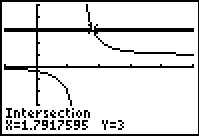
\includegraphics[width=2in]{./ExpLogsGraphics/ExpEqns08.jpg} \\

& $y = f(x) = \frac{e^{x}}{e^{x} - 4}$ \\
& \boldmath $y = g(x) = 3$

\end{tabular}

\end{center}


\item  As before, we start solving $x e^{2x} < 4x$ by getting $0$ on one side of the inequality, $x e^{2x} - 4x < 0$.   We set $r(x) = xe^{2x} - 4x$ and since there are no denominators, even-indexed radicals, or logs, the domain of $r$ is all real numbers.  Setting $r(x) = 0$  produces $x e^{2x} - 4x  = 0$. We factor to get $x \left(e^{2x} - 4\right)  = 0$ which gives $x=0$ or $e^{2x} - 4 = 0$.  To solve the latter, we isolate the exponential and take logs to get $2x = \ln(4)$, or $x = \frac{\ln(4)}{2} = \ln(2)$.  (Can you explain the last equality using properties of logs?)  As in the previous example, we need to be careful about choosing test values.  Since $\ln(1) = 0$, we choose $\ln\left(\frac{1}{2}\right)$, $\ln\left(\frac{3}{2}\right)$ and $\ln(3)$.  Evaluating,\footnote{A calculator can be used at this point. As usual, we proceed without apologies, with the analytical method.} we get 

\[\begin{array}{rclr}

r\left(\ln\left(\frac{1}{2}\right)\right) & = & \ln\left(\frac{1}{2}\right) e^{2\ln\left(\frac{1}{2}\right)} - 4\ln\left(\frac{1}{2}\right) & \\

&= & \ln\left(\frac{1}{2}\right)e^{\ln\left(\frac{1}{2}\right)^2}- 4\ln\left(\frac{1}{2}\right) & \text{Power Rule} \\

& = & \ln\left(\frac{1}{2}\right)e^{\ln\left(\frac{1}{4}\right)}- 4\ln\left(\frac{1}{2}\right) & \\

& = & \frac{1}{4}  \ln\left(\frac{1}{2}\right) - 4  \ln\left(\frac{1}{2}\right) =  -\frac{15}{4} \ln\left(\frac{1}{2}\right) & \end{array}\] 

Since $\frac{1}{2} < 1$, $ \ln\left(\frac{1}{2}\right) < 0$ and we get $r(\ln\left(\frac{1}{2}\right))$ is $(+)$, so $r(x) < 0$ on $(0 ,\ln(2))$.  The calculator confirms that the graph of $f(x) = x e^{2x} $ is below the graph of $g(x) = 4x$ on these intervals.\footnote{Note: $\ln(2) \approx 0.693$.}
\enlargethispage{.5in}

\begin{center}

\begin{tabular}{m{2in}c}

\begin{mfpic}[10]{-5}{5}{-1}{2}
\arrow \reverse \arrow \polyline{(-5,0),(5,0)}
\xmarks{-2,2}
\tlabel[cc](-3.5,1){$(+)$}
\tlabel[cc](-2,-1){$0$}
\tlabel[cc](-2,1){0}
\tlabel[cc](0,1){$(-)$}
\tlabel[cc](2,-1){$\ln(2)$}
\tlabel[cc](2,1){$0$}
\tlabel[cc](3.5,1){$(+)$}
\end{mfpic}

& 

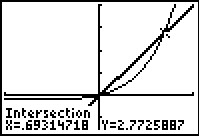
\includegraphics[width=2in]{./ExpLogsGraphics/ExpEqns09.jpg} \\

& $y=f(x) =x e^{2x}$  and \boldmath $y = g(x) = 4x$ \\

\end{tabular}

\end{center}

\end{enumerate}

\qed

\end{ex}

\begin{ex}  Recall from Example \ref{exptempex} that the temperature of coffee $T$ (in degrees Fahrenheit) $t$ minutes after it is served can be modeled by $T(t) = 70 + 90 e^{-0.1 t}$.  When will the coffee be warmer than $100^{\circ}\mbox{F}$?
\smallskip

{\bf Solution.}  We need to find when $T(t) > 100$, or in other words, we need to solve the inequality  $70 + 90 e^{-0.1 t} > 100$.  Getting $0$ on one side of the inequality, we have  $90 e^{-0.1 t} - 30 > 0$, and we set $r(t) = 90 e^{-0.1 t} - 30$.  The domain of $r$ is artificially restricted due to the context of the problem to   $[0, \infty)$, so we proceed to find the zeros of $r$.  Solving $90 e^{-0.1 t} - 30=0$ results in $e^{-0.1t} = \frac{1}{3}$ so that $t = -10\ln\left(\frac{1}{3}\right)$ which, after a quick application of the Power Rule leaves us with $t = 10 \ln(3)$.  If we wish to avoid using the calculator to choose test values, we note that since $1 < 3$, $0 = \ln(1) < \ln(3)$ so that $10\ln(3) > 0$.  So we choose $t = 0$ as a test value in $[0, 10 \ln(3))$.  Since $3 < 4$, $10 \ln(3) < 10 \ln(4)$, so the latter is our choice of a test value for the interval $(10 \ln(3), \infty)$.  Our sign diagram is below, and next to it is our graph of $y=T(t)$ from Example  \ref{exptempex} with the horizontal line $y = 100$.   

\begin{center}

\begin{tabular}{m{0.5in}m{2.5in}m{2.5in}}

&

\begin{mfpic}[10]{0}{8}{-2}{2}
\arrow \polyline{(0,0), (8,0)}
\xmarks{0,4}
\tlabel[cc](0,-1){$0$}
\tlabel[cc](0,1){$(+)$}
\tlabel[cc](4,-1){\scriptsize $10 \ln(3)$}
\tlabel[cc](4,1){$0$}
\tlabel[cc](6,1){$(-)$}
\end{mfpic}

& 

\begin{mfpic}[10]{-1}{11}{-1}{10}
\point[2pt]{(0,8)}
\dashed \polyline{(-1,3.5),(11,3.5)}
\axes
\tlabel[cc](9,2.5){\tiny H.A. $y=70$}
\tlabel[cc](9,5.5){\tiny $y=100$}
\tlabel[cc](11,-0.5){\tiny $t$}
\tlabel[cc](0.5,10){\tiny $y$}
\tcaption{\scriptsize $y = T(t)$}
\ymarks{1,2,3,4,5,6,7,8,9}
\xmarks{1,2,3,4,5,6,7,8,9,10}
\tlpointsep{4pt}
\axislabels {x}{{\tiny $2$} 1, {\tiny $4$} 2, {\tiny $6$} 3, {\tiny $8$} 4,{\tiny $10$} 5, {\tiny $12$} 6, {\tiny $14$} 7, {\tiny $16$} 8, {\tiny $18$} 9, {\tiny $20$} 10}
\axislabels {y}{{\tiny $20$} 1, {\tiny $40$} 2, {\tiny $60$} 3,{\tiny $80$} 4, {\tiny $120$} 6,{\tiny $140$} 7, {\tiny $160$} 8, {\tiny $180$} 9}
\arrow \function{0, 10, 0.1}{(90*exp(0-0.2*x)+70)/20}
\penwd{1.1pt}
\arrow \reverse \arrow \polyline{(-1,5),(11,5)}
\end{mfpic} \\

\end{tabular}

\end{center}

In order to interpret what this means in the context of the real world, we need a reasonable approximation of the number $10 \ln(3) \approx 10.986$.  This means it takes approximately $11$ minutes for the coffee to cool to $100^{\circ}\mbox{F}$.  Until then, the coffee is warmer than that.\footnote{Critics may point out that since we needed to use the calculator to interpret our answer anyway, why not use it earlier to simplify the computations? It is a fair question which we answer unfairly:  it's our book.} \qed
\end{ex}

We close this section by finding the inverse of a function which is a composition of a rational function with an exponential function.

\begin{ex}  \label{expfracinverse} The function $f(x) = \dfrac{5e^{x}}{e^{x}+1}$ is one-to-one.  Find a formula for $f^{-1}(x)$ and check your answer graphically using your calculator.

{\bf Solution.}  We start by writing $y=f(x)$, and interchange the roles of $x$ and $y$.  To solve for $y$, we first clear denominators and then isolate the exponential function.

\[ \begin{array}{rclr}
y & = & \dfrac{5e^{x}}{e^{x}+1} & \\ [12pt]
x & = & \dfrac{5e^{y}}{e^{y}+1} & \mbox{Switch $x$ and $y$} \\ [12pt]
x \left(e^{y}+1\right) & = & 5e^{y} & \\ [4pt]
x e^{y}+x & = & 5e^{y} & \\ [4pt]
x & = & 5e^{y} - x e^{y} & \\ [4pt]
x & = & e^{y}(5 - x) & \\ [4pt]
e^{y}& = & \dfrac{x}{5-x} & \\[12pt]
\ln\left(e^{y}\right) & = & \ln\left(\dfrac{x}{5-x}\right) & \\[12pt]
y & = & \ln\left(\dfrac{x}{5-x}\right) & \\
\end{array}\]

We claim $f^{-1}(x) = \ln\left(\frac{x}{5-x}\right)$.  To verify this analytically, we would need to verify the compositions $\left(f^{-1} \circ f\right)(x) = x$ for all $x$ in the domain of $f$ and that $\left(f \circ f^{-1}\right)(x) = x$ for all $x$ in the domain of $f^{-1}$.  We leave this to the reader.  To verify our solution graphically, we graph $y = f(x) = \frac{5e^{x}}{e^{x}+1}$ and $y = g(x) = \ln\left(\frac{x}{5-x}\right)$ on the same set of axes and observe the symmetry about the line $y=x$.  Note the domain of $f$ is the range of $g$ and vice-versa.

\begin{center}
\begin{tabular}{c}

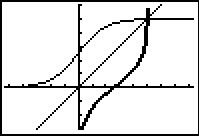
\includegraphics[width=2in]{./ExpLogsGraphics/ExpEqns10.jpg} \\

$y = f(x) = \frac{5e^{x}}{e^{x}+1}$ and \boldmath $y = g(x) = \ln\left(\frac{x}{5-x}\right)$ \\

\end{tabular}
\end{center}

\qed

\end{ex}

\newpage

\subsection{Exercises}


In Exercises \ref{expeqnfirst} - \ref{expeqnlast}, solve the equation analytically.

\begin{multicols}{3}
\begin{enumerate}

\item $2^{4x} = 8$  \label{expeqnfirst} 
\item $3^{(x - 1)} = 27$  
\item $5^{2x-1} = 125$ 

\setcounter{HW}{\value{enumi}}
\end{enumerate}
\end{multicols}

\begin{multicols}{3}
\begin{enumerate}
\setcounter{enumi}{\value{HW}}

\item $4^{2x} = \frac{1}{2}$
\item $8^{x} = \frac{1}{128}$ 
\item $2^{(x^{3} - x)} = 1$ 

\setcounter{HW}{\value{enumi}}
\end{enumerate}
\end{multicols}

\begin{multicols}{3}
\begin{enumerate}
\setcounter{enumi}{\value{HW}}

\item $3^{7x} = 81^{4-2x}$ 
\item $9 \cdot 3^{7x} = \left(\frac{1}{9}\right)^{2x}$ 
\item $3^{2x} = 5$ 

\setcounter{HW}{\value{enumi}}
\end{enumerate}
\end{multicols}

\begin{multicols}{3}
\begin{enumerate}
\setcounter{enumi}{\value{HW}}

\item $5^{-x} = 2$ 
\item $5^{x} = -2$  
\item $3^{(x - 1)} = 29$  

\setcounter{HW}{\value{enumi}}
\end{enumerate}
\end{multicols}

\begin{multicols}{3}
\begin{enumerate}
\setcounter{enumi}{\value{HW}}

\item $(1.005)^{12x} = 3$
\item $e^{-5730k} = \frac{1}{2}$ 
\item $2000e^{0.1t} = 4000$  

\setcounter{HW}{\value{enumi}}
\end{enumerate}
\end{multicols}

\begin{multicols}{3}
\begin{enumerate}
\setcounter{enumi}{\value{HW}}


\item $500\left(1-e^{2x}\right) = 250$
\item $70 + 90e^{-0.1t} = 75$ 
\item $30-6e^{-0.1x}=20$ 


\setcounter{HW}{\value{enumi}}
\end{enumerate}
\end{multicols}

\begin{multicols}{3}
\begin{enumerate}
\setcounter{enumi}{\value{HW}}

\item $\dfrac{100e^{x}}{e^{x}+2}=50$ 
\item $\dfrac{5000}{1+2e^{-3t}}=2500$ 
\item $\dfrac{150}{1 + 29e^{-0.8t}} = 75$ 


\setcounter{HW}{\value{enumi}}
\end{enumerate}
\end{multicols}

\begin{multicols}{3}
\begin{enumerate}
\setcounter{enumi}{\value{HW}}

\item $25\left(\frac{4}{5}\right)^{x} = 10$  

\item $e^{2x} = 2e^{x}$ 
\item  $7e^{2x} = 28e^{-6x}$ 

\setcounter{HW}{\value{enumi}}
\end{enumerate}
\end{multicols}

\begin{multicols}{3}
\begin{enumerate}
\setcounter{enumi}{\value{HW}}

\item $3^{(x - 1)} = 2^{x}$ 
\item $3^{(x - 1)} = \left(\frac{1}{2}\right)^{(x + 5)}$ 
\item  $7^{3+7x} = 3^{4-2x}$  

\setcounter{HW}{\value{enumi}}
\end{enumerate}
\end{multicols}

\begin{multicols}{3}
\begin{enumerate}
\setcounter{enumi}{\value{HW}}

\item $e^{2x} - 3e^{x}-10=0$ %Ans $x=\ln(5)$
\item $e^{2x} = e^{x}+6$ %Ans $x=\ln(2)$
\item $4^{x} + 2^{x} = 12$ %Ans $x=\frac{\ln(3)}{\ln(2)}$


\setcounter{HW}{\value{enumi}}
\end{enumerate}
\end{multicols}

\begin{multicols}{3}
\begin{enumerate}
\setcounter{enumi}{\value{HW}}

\item $e^{x}-3e^{-x}=2$ %Ans $x=\ln(3)$
\item $e^{x}+15e^{-x}=8$ %Ans $x=\ln(2)$, $\ln(5)$
\item $3^{x}+25\cdot3^{-x}=10$ %Ans $x=\frac{\ln(5)}{\ln(3)}$
\label{expeqnlast} 

\setcounter{HW}{\value{enumi}}
\end{enumerate}
\end{multicols}



In Exercises \ref{expineqfirst} - \ref{expineqlast}, solve the inequality analytically.

\begin{multicols}{2} 
\begin{enumerate}
\setcounter{enumi}{\value{HW}}

\item $e^{x} > 53$ \label{expineqfirst} 
\item $1000\left(1.005\right)^{12t} \geq 3000$ 

\setcounter{HW}{\value{enumi}}
\end{enumerate}
\end{multicols}

\begin{multicols}{2} 
\begin{enumerate}
\setcounter{enumi}{\value{HW}}

\item $2^{(x^{3} - x)} < 1$
\item $25\left(\frac{4}{5}\right)^{x} \geq 10$

\setcounter{HW}{\value{enumi}}
\end{enumerate}
\end{multicols}

\begin{multicols}{2} 
\begin{enumerate}
\setcounter{enumi}{\value{HW}}

\item $\dfrac{150}{1 + 29e^{-0.8t}} \leq 130$

\item $\vphantom{\dfrac{150}{1 + 29e^{-0.8t}}} 70 + 90e^{-0.1t} \leq 75$ \label{expineqlast}

\setcounter{HW}{\value{enumi}}
\end{enumerate}
\end{multicols}


In Exercises \ref{calcexpineqfirst} - \ref{calcexpineqlast},  use your calculator to help you solve the equation or  inequality.

\begin{multicols}{3} 
\begin{enumerate}
\setcounter{enumi}{\value{HW}}

\item $2^{x} = x^2$ \label{calcexpineqfirst} 
\item $e^{x} = \ln(x) + 5$   
\item $e^{\sqrt{x}} = x + 1$ 



\setcounter{HW}{\value{enumi}}
\end{enumerate}
\end{multicols}

\begin{multicols}{3} 
\begin{enumerate}
\setcounter{enumi}{\value{HW}}


\item $e^{-x} - xe^{-x} \geq 0$
\item $3^{(x - 1)} < 2^{x}$ 
\item $e^{x} < x^{3} - x$ \label{calcexpineqlast} 


\setcounter{HW}{\value{enumi}}
\end{enumerate}
\end{multicols}


\begin{enumerate}
\setcounter{enumi}{\value{HW}}

\item \label{onetoonelogexercise} Since $f(x) = \ln(x)$ is a strictly increasing function, if $0 < a < b$ then $\ln(a) < \ln(b)$.  Use this fact to solve the inequality $e^{(3x - 1)} > 6$ without a sign diagram. Use this technique to solve the inequalities in Exercises \ref{expineqfirst} - \ref{expineqlast}. (NOTE:  Isolate the exponential function first!)

\item \label{hyperbolicsine} Compute the inverse of $f(x) = \dfrac{e^{x} - e^{-x}}{2}$.  State the domain and range of both $f$ and $f^{-1}$. 

\item In Example \ref{expfracinverse}, we found that the inverse of $f(x) = \dfrac{5e^{x}}{e^{x}+1}$ was $f^{-1}(x) = \ln\left(\dfrac{x}{5-x}\right)$ but we left a few loose ends for you to tie up.  

\begin{enumerate}

\item Show that $\left(f^{-1} \circ f\right)(x) = x$ for all $x$ in the domain of $f$ and that $\left(f \circ f^{-1}\right)(x) = x$ for all $x$ in the domain of $f^{-1}$.

\item Find the range of $f$ by finding the domain of $f^{-1}$.

\item Let $g(x) = \dfrac{5x}{x+1}$ and $h(x) = e^{x}$.  Show that $f = g \circ h$ and that $(g \circ h)^{-1} = h^{-1} \circ g^{-1}$. 
(We know this is true in general by Exercise \ref{fcircginverse} in Section \ref{InverseFunctions}, but it's nice to see a specific example of the property.)

\end{enumerate}

\item With the help of your classmates, solve the inequality $e^{x} > x^{n}$ for a variety of natural numbers $n$.  What might you conjecture about the ``speed'' at which $f(x) = e^{x}$ grows versus any polynomial?

\end{enumerate}

\newpage

\subsection{Answers}


\begin{multicols}{3}
\begin{enumerate}

\item $x = \frac{3}{4}$
\item $x = 4$
\item $x=2$

\setcounter{HW}{\value{enumi}}
\end{enumerate}
\end{multicols}

\begin{multicols}{3}
\begin{enumerate}
\setcounter{enumi}{\value{HW}}

\item $x = -\frac{1}{4}$
\item $x = -\frac{7}{3}$
\item $x = -1, \, 0, \, 1$

\setcounter{HW}{\value{enumi}}
\end{enumerate}
\end{multicols}

\begin{multicols}{3}
\begin{enumerate}
\setcounter{enumi}{\value{HW}}

\item $x = \frac{16}{15}$
\item $x=-\frac{2}{11}$
\item $x = \frac{\ln(5)}{2\ln(3)}$

\setcounter{HW}{\value{enumi}}
\end{enumerate}
\end{multicols}

\begin{multicols}{3}
\begin{enumerate}
\setcounter{enumi}{\value{HW}}

\item $x = -\frac{\ln(2)}{\ln(5)}$
\item No solution.
\item $x = \frac{\ln(29) + \ln(3)}{\ln(3)}$

\setcounter{HW}{\value{enumi}}
\end{enumerate}
\end{multicols}

\begin{multicols}{3}
\begin{enumerate}
\setcounter{enumi}{\value{HW}}

\item $x = \frac{\ln(3)}{12\ln(1.005)}$
\item $k = \frac{\ln\left(\frac{1}{2}\right)}{-5730} = \frac{\ln(2)}{5730} $
\item $t=\frac{\ln(2)}{0.1} = 10\ln(2)$

\setcounter{HW}{\value{enumi}}
\end{enumerate}
\end{multicols}

\begin{multicols}{2}
\begin{enumerate}
\setcounter{enumi}{\value{HW}}


\item $x=\frac{1}{2}\ln\left(\frac{1}{2}\right) = -\frac{1}{2}\ln(2)$
\item $t = \frac{\ln\left(\frac{1}{18}\right)}{-0.1} =10 \ln(18)$



\setcounter{HW}{\value{enumi}}
\end{enumerate}
\end{multicols}

\begin{multicols}{2}
\begin{enumerate}
\setcounter{enumi}{\value{HW}}


\item $x=-10\ln\left(\frac{5}{3}\right) = 10\ln\left(\frac{3}{5}\right)$
\item$x=\ln(2)$

\setcounter{HW}{\value{enumi}}
\end{enumerate}
\end{multicols}

\begin{multicols}{2}
\begin{enumerate}
\setcounter{enumi}{\value{HW}}

\item $t=\frac{1}{3}\ln(2)$
\item $t = \frac{\ln\left(\frac{1}{29}\right)}{-0.8} = \frac{5}{4}\ln(29)$

\setcounter{HW}{\value{enumi}}
\end{enumerate}
\end{multicols}

\begin{multicols}{2}
\begin{enumerate}
\setcounter{enumi}{\value{HW}}

\item $x = \frac{\ln\left(\frac{2}{5}\right)}{\ln\left(\frac{4}{5}\right)} = \frac{\ln(2)-\ln(5)}{\ln(4) - \ln(5)}$

\item $x =  \ln(2)$


\setcounter{HW}{\value{enumi}}
\end{enumerate}
\end{multicols}

\begin{multicols}{2}
\begin{enumerate}
\setcounter{enumi}{\value{HW}}


\item  $x = -\frac{1}{8} \ln\left(\frac{1}{4} \right) = \frac{1}{4}\ln(2)$

\item $x = \frac{\ln(3)}{\ln(3) - \ln(2)}$

\setcounter{HW}{\value{enumi}}
\end{enumerate}
\end{multicols}

\begin{multicols}{2}
\begin{enumerate}
\setcounter{enumi}{\value{HW}}


\item $x = \frac{\ln(3) + 5\ln\left(\frac{1}{2}\right)}{\ln(3) - \ln\left(\frac{1}{2}\right)} = \frac{\ln(3)-5\ln(2)}{\ln(3)+\ln(2)}$
\item  $x = \frac{4 \ln(3) - 3 \ln(7)}{7 \ln(7) + 2 \ln(3)}$

\setcounter{HW}{\value{enumi}}
\end{enumerate}
\end{multicols}

\begin{multicols}{3}
\begin{enumerate}
\setcounter{enumi}{\value{HW}}

\item $x=\ln(5)$
\item $x=\ln(3)$
\item $x=\frac{\ln(3)}{\ln(2)}$


\setcounter{HW}{\value{enumi}}
\end{enumerate}
\end{multicols}

\begin{multicols}{3}
\begin{enumerate}
\setcounter{enumi}{\value{HW}}

\item $x=\ln(3)$
\item $x=\ln(3)$, $\ln(5)$
\item $x=\frac{\ln(5)}{\ln(3)}$


\setcounter{HW}{\value{enumi}}
\end{enumerate}
\end{multicols}

\begin{multicols}{2} 
\begin{enumerate}
\setcounter{enumi}{\value{HW}}

\item $(\ln(53), \infty)$
\item $\left[\frac{\ln(3)}{12\ln(1.005)}, \infty\right)$

\setcounter{HW}{\value{enumi}}
\end{enumerate}
\end{multicols}

\begin{multicols}{2} 
\begin{enumerate}
\setcounter{enumi}{\value{HW}}

\item $(-\infty, -1) \cup (0, 1)$
\item $\left(-\infty, \frac{\ln\left(\frac{2}{5}\right)}{\ln\left(\frac{4}{5}\right)} \right] = \left(-\infty, \frac{\ln(2)-\ln(5)}{\ln(4)-\ln(5)} \right]$

\setcounter{HW}{\value{enumi}}
\end{enumerate}
\end{multicols}

\begin{multicols}{2} 
\begin{enumerate}
\setcounter{enumi}{\value{HW}}

\item $\left(-\infty, \frac{\ln\left(\frac{2}{377}\right)}{-0.8} \right] = \left(-\infty, \frac{5}{4}\ln\left(\frac{377}{2}\right) \right]$
\item $\left[\frac{\ln\left(\frac{1}{18}\right)}{-0.1}, \infty\right) = [10\ln(18), \infty)$

\setcounter{HW}{\value{enumi}}
\end{enumerate}
\end{multicols}

\begin{multicols}{2} 
\begin{enumerate}
\setcounter{enumi}{\value{HW}}

\item $x \approx -0.76666, \, x = 2, \, x = 4$
\item $x \approx 0.01866, \, x \approx 1.7115$


\setcounter{HW}{\value{enumi}}
\end{enumerate}
\end{multicols}

\begin{multicols}{2} 
\begin{enumerate}
\setcounter{enumi}{\value{HW}}

\item $x = 0$
\item $(-\infty, 1]$

\setcounter{HW}{\value{enumi}}
\end{enumerate}
\end{multicols}

\begin{multicols}{2} 
\begin{enumerate}
\setcounter{enumi}{\value{HW}}

\item $\approx (-\infty, 2.7095)$
\item $\approx (2.3217, 4.3717)$


\setcounter{HW}{\value{enumi}}
\end{enumerate}
\end{multicols}


\begin{enumerate}
\setcounter{enumi}{\value{HW}}

\item $x > \frac{1}{3}(\ln(6) + 1)$

\item  $f^{-1} = \ln\left(x + \sqrt{x^{2} + 1}\right)$. Both $f$ and $f^{-1}$ have domain $(-\infty, \infty)$ and range $(-\infty, \infty)$.


\end{enumerate}

\closegraphsfile